\documentclass{beamer}

\usepackage{minted}
\usepackage{tikz}
\usepackage{todonotes}
\usepackage{soul}
\usepackage{graphviz}

\setminted{frame=single}

\usetheme{codecentric}
\author{Markus Hauck}
\institute{codecentric AG}

\title{Functional Web Services}

\hypersetup{colorlinks,linkcolor=beamer@ccblue}

\begin{document}
{
  \usebackgroundtemplate{\includegraphics[width=\paperwidth,height=\paperheight]{../pics/background.png}}
  \begin{frame}[plain,noframenumbering]
    \titlepage{}
  \end{frame}
}

\section{Intro}

\begin{frame}
  \begin{center}
    \huge
    What are we gonna do tonight?
  \end{center}
\end{frame}

\begin{frame}
  \begin{center}
    
\includegraphics[width=0.7\paperwidth]{../pics/pinkybrain.jpg}
  \end{center}
\end{frame}

\begin{frame}
  \frametitle{What are we going to do tonight}
  \begin{minipage}{0.2\linewidth}
    
\includegraphics[width=0.19\linewidth]{../pics/scalpel.png}
  \end{minipage}
  \begin{minipage}{0.7\linewidth}
    \begin{itemize}
    \item explore final encodings
    \item write embedded DSLs
    \item goal: craft beautiful web services
    \end{itemize}
  \end{minipage}
  \vfill
  \begin{center}
    
\includegraphics[height=10mm]{../pics/github.png}
  \end{center}
  \begin{center}
    \url{https://github.com/markus1189/runnersparadise}
  \end{center}
\end{frame}

\begin{frame}
  \frametitle{Before We Start: Embedded DSLs}
  \begin{itemize}
  \item embedded in general purpose language (host language)
  \item separate \textbf{description} of program from
    \textbf{execution}
  \item one of \textbf{the} core principles in FP
  \end{itemize}
\end{frame}

\section{A First DSL}

\begin{frame}[fragile]
  \frametitle{A First DSL}
  \begin{minipage}{0.78\linewidth}
    \begin{itemize}
    \item let's start with our first DSL
    \item arithmetic operations:
      \begin{itemize}
      \item numeric literals
      \item \texttt{addition: e1 + e2}
      \item \texttt{negation: -e}
      \end{itemize}
    \end{itemize}
\begin{minted}{scala}
21 + 21
50 + -(6 + 2)
-(-20 + -20 + -2)
\end{minted}
  \end{minipage}
  \begin{minipage}{0.18\linewidth}
    \begin{center}
      
\includegraphics[width=1.5cm]{../pics/owl.png}
    \end{center}
  \end{minipage}
\end{frame}

\begin{frame}[fragile,fragile]
  \frametitle{Common Approach: Build AST}
\begin{minted}{scala}
sealed trait Exp
case class Lit(x: Int)           extends Exp
case class Neg(e: Exp)           extends Exp
case class Add(e1: Exp, e2: Exp) extends Exp
\end{minted}
  \begin{itemize}
  \item writing a program (syntactic sugar omitted)
  \end{itemize}
\begin{minted}{scala}
// 50 + -(6 + 2)
Add(Lit(50),
    Neg(Add(Lit(6),
            Lit(2))))
\end{minted}
\end{frame}

\begin{frame}[fragile]
  \frametitle{Interpretation}
  \begin{itemize}
  \item we captured the program into a value
  \item able to use different interpreters
  \end{itemize}
\begin{minted}{scala}
def calculate(p: Exp): Int = p match {
  case Lit(x)     => x
  case Neg(e)     => -calculate(e)
  case Add(e1,e2) => calculate(e1) + calculate(e2)
}
def pretty(p: Exp): String = ???
def async(srv: ExpSrv)(p: Exp): Future[Int] = ???
\end{minted}
\end{frame}

\begin{frame}
  \frametitle{Initial Encoding: Drawbacks}
  \begin{itemize}
  \item reify explicitly as AST $\approx{}$ initial encoding
  \item \textcolor{green}{pro}: interpreters can be added easily
  \item \textcolor{red}{con}: try to add multiplication \textbf{as an addon}
    \begin{itemize}
    \item we don't want to change \texttt{Exp}
    \item old interpreters should work as before
    \end{itemize}
  \item spoiler: boils down to the expression problem
  \end{itemize}
\end{frame}

\begin{frame}
  \frametitle{Alternative}
  \begin{itemize}
  \item what if we scratch the whole ``reify as AST'' step?
  \item leads to \textit{final encodings}
  \item \begin{itemize}
    \item no datatype
    \item instead: write type classes
    \item instances = interpreter
    \end{itemize}
  \item let's define another calculator
  \end{itemize}
\end{frame}

\begin{frame}[fragile]
  \frametitle{Final Encoding: Calculator}
\begin{minted}{scala}
sealed trait Exp[A] {
  def lit(x: Int): A
  def neg(e: A): A
  def add(e1: A, e2: A): A
}
\end{minted}
  \begin{itemize}
  \item writing a program
  \end{itemize}
\begin{minted}{scala}
// 50 + -(6 + 2)
def program[A](implicit E: Exp[A]): A = {
  import E._ // for demo
  add(lit(50),
      neg(add(lit(6),
              lit(2))))
}
\end{minted}
\end{frame}

\begin{frame}[fragile]
  \frametitle{Final Encoding: Interpreter}
  \begin{itemize}
  \item define interpreters as instances:
  \end{itemize}
\begin{minted}{scala}
implicit val calc: Exp[Int] = new Exp[Int] {
  def lit(x: Int): Int = x
  def neg(e: Int): Int = -e
  def add(e1: Int, e2: Int): Int = e1 + e2
}
implicit val pretty: Exp[String] = new Exp[String] {
  def lit(x: Int): String = x.shows
  def neg(e: String): String = "-" + e
  def add(e1: String, e2: String) = s"($e1 + $e2)"
}
\end{minted}
\end{frame}

\begin{frame}[fragile]
  \frametitle{Final Encoding: Running}
  \begin{itemize}
  \item now that we have interpreters, we can run our program:
  \end{itemize}
\begin{minted}{scala}
scala> program[Int]
res0: Int = 42
scala> program[String]
res1: String = (50 + -(6 + 2))
\end{minted}
  \begin{itemize}
  \item (please use newtypes for instances)
  \end{itemize}
\end{frame}

\begin{frame}
  \frametitle{Final Encoding: Extension}
  \begin{itemize}
  \item the important part: let's add multiplication
  \item goal: change should not impact existing code
  \end{itemize}
\end{frame}

\begin{frame}[fragile]
  \frametitle{Final Encoding: Multiplication}
  \begin{itemize}
  \item add new typeclass
  \item state required operations
  \item note: independent of the others
  \end{itemize}

\begin{minted}{scala}
sealed trait ExpMul[A] {
  def mul(e1: A, e2: A): A
}
\end{minted}
\end{frame}

\begin{frame}[fragile]
  \frametitle{Final Encoding: Using Multiplication}
\begin{minted}{scala}
def mulProgram[A](
  implicit E1: Exp[A], E2: ExpMul[A]
): A = {
  import E1._, E2._
  // 2 * (1 + (10 + 10))
  mul(lit(2),
      add(lit(1),
          add(lit(10),
              lit(10))))
}
\end{minted}
\end{frame}

\begin{frame}[fragile]
  \frametitle{Final Encoding: Extend Interpreters}
  \begin{itemize}
  \item before we can run this, we need to add the instances
  \end{itemize}
\begin{minted}{scala}
implicit val calc: ExpMul[Int] = new ExpMul[Int] {
  def mul(e1: Int, e2: Int): Int = e1 * e2
}

implicit val pretty: ExpMul[String] =
  new ExpMul[String] {
    def mul(e1: String, e2: String): String =
      s"($e1 * $e2)"
}

\end{minted}
\end{frame}

\begin{frame}[fragile]
  \frametitle{Final Encoding: Execute Multiplication}
\begin{minted}{scala}
scala> mulProgram[Int]
res0: Int = 42
scala> mulProgram[String]
res1: String = "(2 * (1 + (10 + 10)))"
\end{minted}
\end{frame}

\begin{frame}[fragile]
  \setminted{frame=none}
  \frametitle{Review: Final Encoding}
  \begin{minipage}[frame=none]{0.45\linewidth}
\begin{minted}{scala}
sealed trait Exp[A] {
  def lit(x:Int): A
  def neg(e:A): A
  def add(e1 A, e2:A): A
}
\end{minted}
  \end{minipage}
  \begin{minipage}[frame=none]{0.45\linewidth}
\begin{minted}{scala}
new Exp[Int] {
  def lit(x:Int) = x
  def neg(e: Int) -e
  def add(e1:Int,e2:Int) =
    e1 + e2
  }
\end{minted}
  \end{minipage}
  \begin{itemize}
  \item define typeclass for syntax
  \item define instance for semantics
  \item languages are \textbf{independent} and \textbf{composable}
  \item but: no AST\ldots, what about optimizations?
  \end{itemize}
\end{frame}

\begin{frame}
  \frametitle{Final Encoding: Transformations}
  \begin{itemize}
  \item in fact, we can still perform program transformations
  \item example: push down negations
    \begin{itemize}
    \item idea: move all ``negations'' into the leaves
    \item \texttt{-(1 + 2)} $\rightarrow$ \texttt{(-1 + -2)}
    \end{itemize}
  \end{itemize}
\end{frame}

\begin{frame}
  \frametitle{Final Encoding: Transformations}
  \begin{center}
    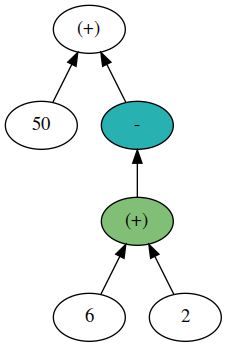
\includegraphics[height=5cm]{../graphs/ast-from.png}
    \hfill
    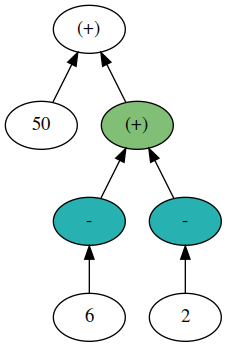
\includegraphics[height=5cm]{../graphs/ast-to.png}
  \end{center}
\end{frame}

\begin{frame}[fragile,fragile,fragile]
  \frametitle{Final Encoding: Transformations}
  \begin{itemize}
  \item we have to make the required context explicit
  \item what do we need for pushing down negations?
  \end{itemize}
\begin{minted}{scala}
sealed trait Ctx
case object P extends Ctx
case object N extends Ctx

// newtype for: Ctx => A
final class Push[A](val run: Ctx => A) extends AnyVal
\end{minted}
\end{frame}

\begin{frame}[fragile]
  \frametitle{Final Encoding: Transformations}
\begin{minted}{scala}
def pushNeg[A](implicit E: Exp[A]): Exp[Push[A]] =
  new Exp[Push[A]] {
    def add(e1: Push[A], e2: Push[A]): Push[A] =
      new Push(ctx => E.add(e1.run(ctx),e2.run(ctx)))

    def neg(e: Push[A]): Push[A] = new Push({
      case P => e.run(N)
      case N => e.run(P)
    })

    def lit(x: Int): Push[A] = new Push({
      case P => E.lit(x)
      case N => E.neg(E.lit(x))
    })
}
\end{minted}
\end{frame}

\begin{frame}[fragile]
  \addtocounter{framenumber}{-1}
  \frametitle{Final Encoding: Transformations}
\begin{minted}{scala}
def pushNeg[A](implicit E: Exp[A]): Exp[Push[A]] =
  new Exp[Push[A]] {
    def add(e1: Push[A], e2: Push[A]): Push[A] =
      new Push(ctx => E.add(e1.run(ctx),e2.run(ctx)))










}
\end{minted}
\end{frame}

\begin{frame}[fragile]
  \addtocounter{framenumber}{-1}
  \frametitle{Final Encoding: Transformations}
\begin{minted}{scala}
def pushNeg[A](implicit E: Exp[A]): Exp[Push[A]] =
  new Exp[Push[A]] {



    def neg(e: Push[A]): Push[A] = new Push({
      case P => e.run(N)
      case N => e.run(P)
    })





}
\end{minted}
\end{frame}

\begin{frame}[fragile]
  \addtocounter{framenumber}{-1}
  \frametitle{Final Encoding: Transformations}
\begin{minted}{scala}
def pushNeg[A](implicit E: Exp[A]): Exp[Push[A]] =
  new Exp[Push[A]] {








    def lit(x: Int): Push[A] = new Push({
      case P => E.lit(x)
      case N => E.neg(E.lit(x))
    })
}
\end{minted}
\end{frame}

\begin{frame}[fragile]
  \addtocounter{framenumber}{-1}
  \frametitle{Final Encoding: Transformations}
\begin{minted}{scala}
def pushNeg[A](implicit E: Exp[A]): Exp[Push[A]] =
  new Exp[Push[A]] {
    def add(e1: Push[A], e2: Push[A]): Push[A] =
      new Push(ctx => E.add(e1.run(ctx),e2.run(ctx)))

    def neg(e: Push[A]): Push[A] = new Push({
      case P => e.run(N)
      case N => e.run(P)
    })

    def lit(x: Int): Push[A] = new Push({
      case P => E.lit(x)
      case N => E.neg(E.lit(x))
    })
}
\end{minted}
\end{frame}

\begin{frame}[fragile]
  \frametitle{Final Encoding: Performing Transformation}
\begin{minted}{scala}
scala> program[String]
res0: String = (50 + -(6 + 2))

scala> program[Push[String]]
res1: Push[String] = ...

scala> program[Push[String]].run(P)
res2: String = (50 + (-6 + -2))
\end{minted}
\end{frame}

\begin{frame}
  \frametitle{Final Encoding: Review}
  \begin{itemize}
  \item we \textbf{can} do transformations after all
  \item (although still not as nice as pattern matching)
  \item extension is possible without adapting existing code
  \item so far, so good
  \end{itemize}
\end{frame}

\begin{frame}
  \frametitle{When You Have A Shiny New Hammer\ldots}
  \begin{minipage}{0.48\linewidth}
  \begin{figure}
    \centering
    
\includegraphics[height=4cm]{../pics/hammer.png}
    \caption{Final Encoding}
  \end{figure}
  \end{minipage}
  \begin{minipage}{0.48\linewidth}
    \begin{figure}
      \centering 
\includegraphics[height=3cm]{../pics/nail.png}
      \caption{???}
    \end{figure}
  \end{minipage}
\end{frame}

\section{Web Services With Http4s}

\begin{frame}
  \begin{center}
    \Huge Web Services with Http4s
  \end{center}
\end{frame}

\begin{frame}{http4s}
  \begin{center}
    
\includegraphics[width=15mm]{../pics/http4s.png}
  \end{center}

  \begin{block}{What is \hyperlink{http://http4s.org/}{http4s}}
    A typeful, purely functional, streaming library for HTTP
    clients and servers in Scala.
  \end{block}
  \begin{itemize}
  \item typeful \textemdash{} self-documentation and compile-time verification
  \item purely functional \textemdash{} promote composability and reasoning
  \item streaming \textemdash{} large payloads in constant space and
    websockets
  \end{itemize}
  \begin{center}
    \alert{(currently being rewritten to use \texttt{cats} and \texttt{fs2})}
  \end{center}

\end{frame}

\begin{frame}[fragile]
  \frametitle{Writing Web Services With Http4s}
  \begin{itemize}
  \item define \texttt{HttpService} using the built-in DSL
  \item \texttt{really} just \texttt{Request => Task[Response]}
  \item (\texttt{Task[A]} is a better\footnote{in the context of FP} \texttt{Future[A]})
  \item define routes via pattern matching:
  \end{itemize}
\begin{minted}{scala}
HttpService {
  case req @ GET -> Root / "hello" =>
    handleHelloWorld(req)
}
\end{minted}
\end{frame}

\section{Runner's Paradise DSL}

\begin{frame}
  \frametitle{Our Domain}
  \begin{center}
    \huge
    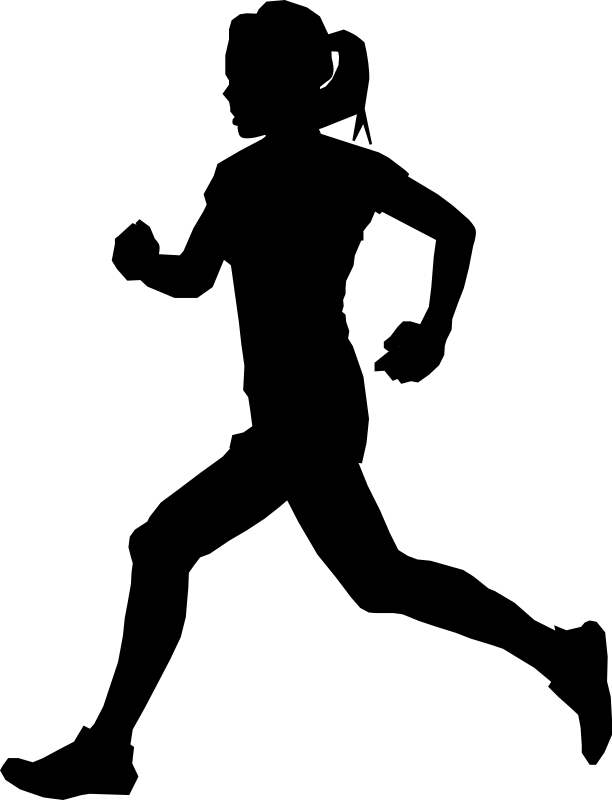
\includegraphics[width=2cm]{../pics/runner.png}
    Runners
    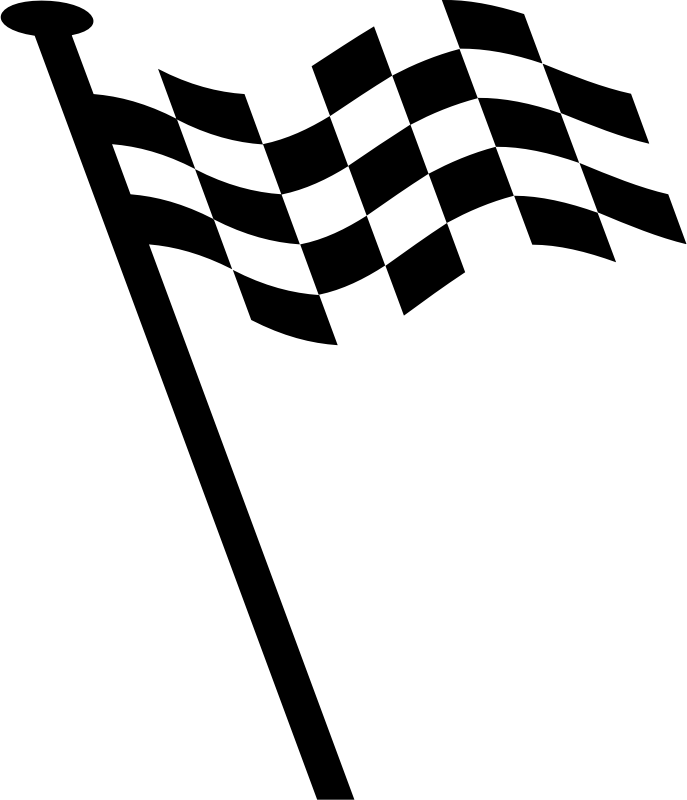
\includegraphics[width=2cm]{../pics/race.png}
    Races
    
\includegraphics[width=2cm]{../pics/registration.png}
    Registrations
  \end{center}
\end{frame}

\begin{frame}[fragile]
  \frametitle{Our API}
\begin{minted}{scala}
GET  "/runner/<runner-id>"
POST "/runner"

GET  "/race/<race-id>"
POST "/race"

GET  "/registration/<race-id>"
PUT  "/registration"
\end{minted}
\end{frame}

\begin{frame}[fragile]
  \frametitle{Our API}
\begin{minted}[fontsize=\small]{scala}
HttpService {

  case GET -> Root / "runner" / RunnerIdVar(v)     => ???
  case req @ POST -> Root / "runner"               => ???

  case GET -> Root / "race" / RaceIdVar(v)         => ???
  case req @ POST -> Root / "race"                 => ???

  case GET -> Root / "registration" / RaceIdVar(v) => ???
  case req @ PUT -> Root / "registration"          => ???

}
\end{minted}
\end{frame}

\begin{frame}
  \frametitle{The Idea}
  \begin{itemize}
  \item define a web service that uses a DSL
  \item each request modeled as a program that is executed
  \end{itemize}
\end{frame}

\begin{frame}[fragile]
  \frametitle{The Runners Paradise DSL}
\begin{minted}{scala}
trait RunnerAlg[F[_]] {
  def saveRunner(runner: Runner): F[Unit]
  def findRunner(id: RunnerId): F[Option[Runner]]
}
\end{minted}
  \begin{itemize}
  \item we use a \textit{higher-kinded} type \texttt{F}
  \item kind: \texttt{* -> *}, i.e.\ it needs another type of kind
    \texttt{*}
  \item results are wrapped in \texttt{F[\_]}
  \item \textit{instances choose the concrete F}
  \end{itemize}
\end{frame}

\begin{frame}[fragile]
  \frametitle{The Runners Paradise DSL}
\begin{minted}{scala}
trait RaceAlg[F[_]] {
  def saveRace(race: Race): F[Unit]
  def findRace(id: RaceId): F[Option[Race]]
}
\end{minted}
\begin{minted}{scala}
trait RegistrationAlg[F[_]] {
  def saveReg(reg: Registration): F[Unit]
  def findReg(id: RaceId): F[Option[Registration]]
}
\end{minted}
\end{frame}

\begin{frame}
  \frametitle{Let's hammer}
  \begin{itemize}
  \item each route leads to a program being executed
  \item the interpreter is left abstract, instantiate when running
  \item let's implement: registration of a runner for a race
  \end{itemize}
\end{frame}

\begin{frame}
  \frametitle{The Runners Pradise DSL: Registrations}
  \begin{itemize}
  \item allow registration of runners for races
  \item if:
    \begin{itemize}
    \item race exists
    \item runner exists
    \item race has free slots
    \end{itemize}
  \item reality: \texttt{Either[RegistrationError,Registration]}
  \end{itemize}
\end{frame}

\begin{frame}
  \frametitle{Fair Warning: Fancy Code Incoming}
  
\includegraphics[width=\textwidth]{../pics/warning.png}
\end{frame}

\begin{frame}[fragile]
  \frametitle{The Runners Paradise DSL}
\begin{minted}[fontsize=\footnotesize]{scala}
def registerOpt[F[_]:Monad:RunnerAlg:RaceAlg:RegistrationAlg](
      runnerId: RunnerId,
      raceId: RaceId): F[Option[Registration]] = {

    val M = Monad[OptionT[F, ?]]

    for {
      runner <- OptionT(RunnerAlg().findRunner(runnerId))
      race   <- OptionT(RaceAlg().findRace(raceId))
      reg    <- OptionT(RegistrationAlg().findReg(raceId)).
                  orElse(M.point(Registration(race, Set())))
      newReg <- OptionT(reg.add(runner).pure[F])
      _      <- OptionT(RegistrationAlg().saveReg(newReg).
                  map(Option(_)))
    } yield newReg
  }.run
\end{minted}
\end{frame}

\begin{frame}[fragile]
  \addtocounter{framenumber}{-1}
  \frametitle{Registration Program}
\begin{minted}{scala}
def registerOpt[F[_]:             // still abstract
                Monad:            // flatMap
                RunnerAlg:        // runners
                RaceAlg:          // races
                RegistrationAlg]( // registrations
  runnerId: RunnerId,             // runner id
  raceId: RaceId                  // race id
): F[Option[Registration]]        // wrapped in F
\end{minted}
\end{frame}

\begin{frame}[fragile]
  \addtocounter{framenumber}{-1}
  \frametitle{The Runners Paradise DSL}
\begin{minted}[fontsize=\footnotesize]{scala}
def registerOpt[F[_]:Monad:RunnerAlg:RaceAlg:RegistrationAlg](
      runnerId: RunnerId,
      raceId: RaceId): F[Option[Registration]] = {

    val M = Monad[OptionT[F, ?]]

//  for {
//    runner <- OptionT(RunnerAlg().findRunner(runnerId))
//    race   <- OptionT(RaceAlg().findRace(raceId))
//    reg    <- OptionT(RegistrationAlg().findReg(raceId)).
//                orElse(M.point(Registration(race, Set())))
//    newReg <- OptionT(reg.add(runner).pure[F])
//    _      <- OptionT(RegistrationAlg().saveReg(newReg).
//                map(Option(_)))
//  } yield newReg
  }.run
\end{minted}
\end{frame}

\begin{frame}[fragile]
  \addtocounter{framenumber}{-1}
  \frametitle{The Runners Paradise DSL}
\begin{minted}[fontsize=\footnotesize]{scala}
def registerOpt[F[_]:Monad:RunnerAlg:RaceAlg:RegistrationAlg](
      runnerId: RunnerId,
      raceId: RaceId): F[Option[Registration]] = {

    val M = Monad[OptionT[F, ?]]

//  for {
      runner <- OptionT(RunnerAlg().findRunner(runnerId))
//    race   <- OptionT(RaceAlg().findRace(raceId))
//    reg    <- OptionT(RegistrationAlg().findReg(raceId)).
//                orElse(M.point(Registration(race, Set())))
//    newReg <- OptionT(reg.add(runner).pure[F])
//    _      <- OptionT(RegistrationAlg().saveReg(newReg).
//                map(Option(_)))
//  } yield newReg
  }.run
\end{minted}
\end{frame}

\begin{frame}[fragile]
  \addtocounter{framenumber}{-1}
  \frametitle{The Runners Paradise DSL}
\begin{minted}[fontsize=\footnotesize]{scala}
def registerOpt[F[_]:Monad:RunnerAlg:RaceAlg:RegistrationAlg](
      runnerId: RunnerId,
      raceId: RaceId): F[Option[Registration]] = {

    val M = Monad[OptionT[F, ?]]

//  for {
//    runner <- OptionT(RunnerAlg().findRunner(runnerId))
      race   <- OptionT(RaceAlg().findRace(raceId))
//    reg    <- OptionT(RegistrationAlg().findReg(raceId)).
//                orElse(M.point(Registration(race, Set())))
//    newReg <- OptionT(reg.add(runner).pure[F])
//    _      <- OptionT(RegistrationAlg().saveReg(newReg).
//                map(Option(_)))
//  } yield newReg
  }.run
\end{minted}
\end{frame}

\begin{frame}[fragile]
  \addtocounter{framenumber}{-1}
  \frametitle{The Runners Paradise DSL}
\begin{minted}[fontsize=\footnotesize]{scala}
def registerOpt[F[_]:Monad:RunnerAlg:RaceAlg:RegistrationAlg](
      runnerId: RunnerId,
      raceId: RaceId): F[Option[Registration]] = {

    val M = Monad[OptionT[F, ?]]

//  for {
//    runner <- OptionT(RunnerAlg().findRunner(runnerId))
//    race   <- OptionT(RaceAlg().findRace(raceId))
      reg    <- OptionT(RegistrationAlg().findReg(raceId)).
                  orElse(M.point(Registration(race, Set())))
//    newReg <- OptionT(reg.add(runner).pure[F])
//    _      <- OptionT(RegistrationAlg().saveReg(newReg).
//                map(Option(_)))
//  } yield newReg
  }.run
\end{minted}
\end{frame}

\begin{frame}[fragile]
  \addtocounter{framenumber}{-1}
  \frametitle{The Runners Paradise DSL}
\begin{minted}[fontsize=\footnotesize]{scala}
def registerOpt[F[_]:Monad:RunnerAlg:RaceAlg:RegistrationAlg](
      runnerId: RunnerId,
      raceId: RaceId): F[Option[Registration]] = {

    val M = Monad[OptionT[F, ?]]

//  for {
//    runner <- OptionT(RunnerAlg().findRunner(runnerId))
//    race   <- OptionT(RaceAlg().findRace(raceId))
//    reg    <- OptionT(RegistrationAlg().findReg(raceId)).
//                orElse(M.point(Registration(race, Set())))
      newReg <- OptionT(reg.add(runner).pure[F])
//    _      <- OptionT(RegistrationAlg().saveReg(newReg).
//                map(Option(_)))
//  } yield newReg
  }.run
\end{minted}
\end{frame}

\begin{frame}[fragile]
  \addtocounter{framenumber}{-1}
  \frametitle{The Runners Paradise DSL}
\begin{minted}[fontsize=\footnotesize]{scala}
def registerOpt[F[_]:Monad:RunnerAlg:RaceAlg:RegistrationAlg](
      runnerId: RunnerId,
      raceId: RaceId): F[Option[Registration]] = {

    val M = Monad[OptionT[F, ?]]

//  for {
//    runner <- OptionT(RunnerAlg().findRunner(runnerId))
//    race   <- OptionT(RaceAlg().findRace(raceId))
//    reg    <- OptionT(RegistrationAlg().findReg(raceId)).
//                orElse(M.point(Registration(race, Set())))
//    newReg <- OptionT(reg.add(runner).pure[F])
      _      <- OptionT(RegistrationAlg().saveReg(newReg).
                  map(Option(_)))
//  } yield newReg
  }.run
\end{minted}
\end{frame}

\begin{frame}[fragile]
  \addtocounter{framenumber}{-1}
  \frametitle{The Runners Paradise DSL}
\begin{minted}[fontsize=\footnotesize]{scala}
def registerOpt[F[_]:Monad:RunnerAlg:RaceAlg:RegistrationAlg](
      runnerId: RunnerId,
      raceId: RaceId): F[Option[Registration]] = {

    val M = Monad[OptionT[F, ?]]

    for {
      runner <- OptionT(RunnerAlg().findRunner(runnerId))
      race   <- OptionT(RaceAlg().findRace(raceId))
      reg    <- OptionT(RegistrationAlg().findReg(raceId)).
                  orElse(M.point(Registration(race, Set())))
      newReg <- OptionT(reg.add(runner).pure[F])
      _      <- OptionT(RegistrationAlg().saveReg(newReg).
                  map(Option(_)))
    } yield newReg
  }.run
\end{minted}
\end{frame}

\begin{frame}
  \frametitle{Getting More Concrete: Instances}
  \begin{itemize}
  \item to actually run programs, we need to have instances
  \item need to satisfy \texttt{all} constraints
  \item pure in-memory, cassandra, postgres, redis, \dots{}
  \end{itemize}
\end{frame}

\begin{frame}[fragile,fragile]
  \frametitle{Instances for our DSL}
\begin{minted}{scala}
class Cass[A](
  val value: ReaderT[Task, RunnersParadiseDb, A]
) extends AnyVal {
  def run: RunnersParadiseDb => Task[A] = value.run
}
\end{minted}
  \begin{itemize}
  \item \texttt{RunnersParadiseDb => Task[A]}
  \item given a connection to the DB, asynchronous results
  \end{itemize}
\end{frame}

\begin{frame}[fragile,fragile]
  \frametitle{Instances for our DSL}
\begin{minted}{scala}
class Cass[A](
  val value: ReaderT[Task, RunnersParadiseDb, A]
) extends AnyVal {
  def run: RunnersParadiseDb => Task[A] = value.run
}
\end{minted}
  \vfill
\begin{minted}{scala}
def saveRunner(runner: Runner): Cass[Unit] =
  new Cass(ReaderT(_.runners.save(runner).void))
\end{minted}
\end{frame}

\section{Final Encodings and http4s}

\begin{frame}[fragile]
  \frametitle{Putting It Together}
  \begin{itemize}
  \item remember signature of routes?
  \end{itemize}
\begin{minted}{scala}
Request => Task[Response]
\end{minted}
  \begin{itemize}
  \item at the end our program \textbf{has} to produce a \texttt{Task}
  \item but we don't want to be limited by this
  \end{itemize}
\end{frame}

\begin{frame}[fragile]
  \frametitle{The RaceRegistrationService}
\begin{minted}{scala}
case class Register(runner: RunnerId, race: RaceId)
class RaceRegistrationService[F[_]:Monad
                                  :RunnerAlg
                                  :RaceAlg
                                  :RegistrationAlg](
  natF: F ~> Task) {

  def service: HttpService = {
    def route = HttpService {
      // ...
      case req @ PUT -> Root / "registration" =>
        handleRegistration(req)
    }
  }
  // private def handleRegistration ...
}
\end{minted}
\end{frame}

\begin{frame}[fragile]
  \addtocounter{framenumber}{-1}
  \frametitle{The RaceRegistrationService}
\begin{minted}{scala}
case class Register(runner: RunnerId, race: RaceId)
class RaceRegistrationService[F[_]:Monad
                                  :RunnerAlg
                                  :RaceAlg
                                  :RegistrationAlg](
  natF: F ~> Task) {

  private def handleRegistration(req: Req) = {
    req.decodeWith(jsonOf[Register]) { reg =>
      Programs.register[F](
        reg.number,
        reg.race
      )
    }
  }
}
\end{minted}
\end{frame}

\begin{frame}
  \frametitle{So what?}
  \begin{itemize}
  \item okay we added a LOT of abstraction in our web service\ldots
  \item why should we do that?
    \begin{itemize}
    \item composability
    \item testability
    \end{itemize}
  \end{itemize}
\end{frame}

\begin{frame}
  \frametitle{Composablity}
  \begin{itemize}
  \item we can choose interpreters and also mix them as we want:
  \item remember push down negations?
    \begin{itemize}
    \item logging
    \item security
    \item timeouts
    \item tracing
    \end{itemize}
  \end{itemize}
\end{frame}

\begin{frame}
  \frametitle{Testability}
  \begin{itemize}
  \item use in-memory interpreter by only changing the type parameter
  \item formulate laws on our type classes
  \item use ScalaCheck to check for all instances (Cassandra, Redis,
    \ldots)
  \item nice separation of domain logic that should not use the DSL
  \end{itemize}
\end{frame}

\begin{frame}
  \frametitle{Review of Final Encodings}
  \begin{itemize}
  \item initial encoding: pattern matching and transformations more obvious
  \item final encoding: easier to extend, same expressiveness
  \item btw: nice way to solve \href{https://stackoverflow.com/questions/3596366/what-is-the-expression-problem\#3776140}{expression problem} (exercise)
  \item you can \textit{always} convert between initial and final
  \end{itemize}
\end{frame}

\begin{frame}
  \frametitle{Final Encodings and Free Monads}
  \begin{itemize}
  \item final encoding + higher kinded type constructor\ldots
  \item similar to Free Monads, the latter use an initial encoding
  \item the two are \textit{interchangeable}
    \begin{itemize}
    \item final encoding $\rightarrow$ free monads: type class instance that builds the
      free structure

    \item free monads $\rightarrow$ final encoding: take in an instance and use
      it
    \end{itemize}
  \end{itemize}
\end{frame}

\begin{frame}[fragile]
  \frametitle{Finalizing a Free Monad Program}
\begin{minted}{scala}
def finalize[R, F[_]:Monad:RunnerAlg](
  p: FreeC[RunnerAlgFree, R]): F[R] =

    Free.runFC(p)(new (RunnerAlgFree ~> F) {
    def apply[A](fa: RunnerAlgFree[A]): F[A] =
      fa match {
        case SaveRunner(runner) =>
          RunnerAlg[F].saveRunner(runner)
        case FindRunner(id) =>
          RunnerAlg[F].findRunner(id)

      }})
\end{minted}
\end{frame}

\begin{frame}
  \frametitle{Further References}
  \begin{itemize}
  \item Oleg Kiselyov: Lecture notes on
    \href{http://okmij.org/ftp/tagless-final/course/lecture.pdf}{Typed
      Tagless Final Interpreters}
  \item Runner's Paradise Code:
    \url{https://github.com/markus1189/runnersparadise}
  \item http4s: \url{http://http4s.org/}
  \end{itemize}
\end{frame}

\begin{frame}
  \frametitle{Questions}
  \begin{center}
    
\includegraphics[width=0.5\textwidth]{../pics/questions.png}
  \end{center}
\end{frame}

\end{document}
